\documentclass[border=4pt]{standalone}
\usepackage{fontspec}
\IfFileExists{fonts/times.ttf}{
  \setmainfont{times.ttf}[Path=fonts/,
    BoldFont=timesbd.ttf, ItalicFont=timesi.ttf, BoldItalicFont=timesbi.ttf]
}{\usepackage{mathptmx}}
\usepackage{tikz}
\usetikzlibrary{arrows.meta,positioning,fit,backgrounds}
\begin{document}
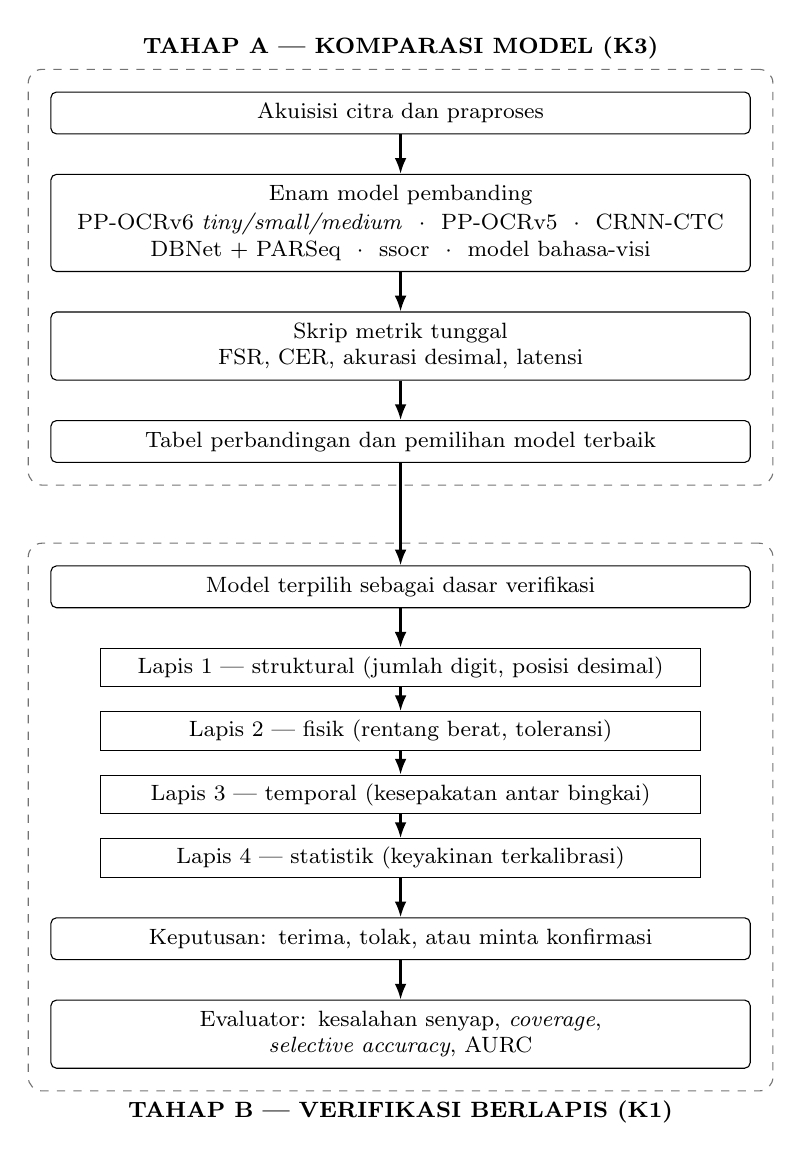
\begin{tikzpicture}[
  node distance=0.5cm,
  blok/.style={rectangle, draw, rounded corners=2pt, align=center,
               text width=8.6cm, inner sep=4pt, font=\footnotesize},
  lapis/.style={rectangle, draw, align=center, inner sep=3pt,
                font=\footnotesize, text width=7.4cm},
  panah/.style={-{Latex[length=2mm]}, thick},
  judul/.style={font=\footnotesize\bfseries, align=center}
]

\node[blok] (akuisisi) {Akuisisi citra dan praproses};
\node[blok, below=of akuisisi] (model)
  {Enam model pembanding\\[1pt]
   PP-OCRv6 \textit{tiny/small/medium} ~$\cdot$~ PP-OCRv5 ~$\cdot$~ CRNN-CTC\\
   DBNet + PARSeq ~$\cdot$~ ssocr ~$\cdot$~ model bahasa-visi};
\node[blok, below=of model] (metrik)
  {Skrip metrik tunggal\\ FSR, CER, akurasi desimal, latensi};
\node[blok, below=of metrik] (tabel)
  {Tabel perbandingan dan pemilihan model terbaik};

\draw[panah] (akuisisi) -- (model);
\draw[panah] (model) -- (metrik);
\draw[panah] (metrik) -- (tabel);

\node[blok, below=1.3cm of tabel] (pilih)
  {Model terpilih sebagai dasar verifikasi};
\node[lapis, below=of pilih] (l1) {Lapis 1 --- struktural (jumlah digit, posisi desimal)};
\node[lapis, below=0.3cm of l1] (l2) {Lapis 2 --- fisik (rentang berat, toleransi)};
\node[lapis, below=0.3cm of l2] (l3) {Lapis 3 --- temporal (kesepakatan antar bingkai)};
\node[lapis, below=0.3cm of l3] (l4) {Lapis 4 --- statistik (keyakinan terkalibrasi)};
\node[blok, below=of l4] (putus)
  {Keputusan: terima, tolak, atau minta konfirmasi};
\node[blok, below=of putus] (eval)
  {Evaluator: kesalahan senyap, \textit{coverage},\\ \textit{selective accuracy}, AURC};

\draw[panah] (tabel) -- (pilih);
\draw[panah] (pilih) -- (l1);
\draw[panah] (l1) -- (l2);
\draw[panah] (l2) -- (l3);
\draw[panah] (l3) -- (l4);
\draw[panah] (l4) -- (putus);
\draw[panah] (putus) -- (eval);

\begin{scope}[on background layer]
  \node[draw=black!55, dashed, rounded corners=5pt, inner sep=8pt,
        fit=(akuisisi)(tabel),
        label={[judul]above:TAHAP A --- KOMPARASI MODEL (K3)}] {};
  \node[draw=black!55, dashed, rounded corners=5pt, inner sep=8pt,
        fit=(pilih)(eval),
        label={[judul]below:TAHAP B --- VERIFIKASI BERLAPIS (K1)}] {};
\end{scope}

\end{tikzpicture}
\end{document}
